\documentclass[12pt]{article}
%[10pt,technote]{IEEEtran}
\usepackage{hyperref}
\usepackage{graphicx}
\usepackage[affil-it]{authblk}
\usepackage{color}
\usepackage{amsgen,amsmath,amstext,amsbsy,amsopn,amssymb}
\usepackage{geometry}
\usepackage{subcaption}
\usepackage{caption}
\usepackage{wrapfig}
\usepackage{comment}
\usepackage{mathrsfs}
\usepackage{upgreek}
\usepackage{amssymb}
\usepackage{textcomp}
\usepackage{amsmath}
\usepackage{tcolorbox}
\usepackage{listings}

%\usepackage{subfigure}
%\usepackage{wraptable}

\geometry{left=2.5cm, right=2.5cm,top=2.5cm,bottom=2.5cm}



\setcounter{secnumdepth}{0}
\title{\bf Homework 2}
\author{Jiani Gao\\jgao30@binghamton.edu}
\affil{Department of Economics, Binghamton University}
\date{\today}
\begin{document}
	\lstset{language=Matlab,%
		%basicstyle=\color{red},
		breaklines=true,%
		morekeywords={matlab2tikz},
		keywordstyle=\color{blue},%
		morekeywords=[2]{1}, keywordstyle=[2]{\color{black}},
		identifierstyle=\color{black},%
		stringstyle=\color{mylilas},
		commentstyle=\color{mygreen},%
		showstringspaces=false,%without this there will be a symbol in the places where there is a space
		numbers=left,%
		numberstyle={\tiny \color{black}},% size of the numbers
		numbersep=9pt, % this defines how far the numbers are from the text
		emph=[1]{for,end,break},emphstyle=[1]\color{red}, %some words to emphasise
		%emph=[2]{word1,word2}, emphstyle=[2]{style},    
	}
	\maketitle
	\newpage
	\tableofcontents
	\newpage
    \section{Question 1}
    Functional equation:\\\\
   $(A_t(S^t)K_t^\alpha+(1-\delta)K_t-K_{t+1})^{-\sigma}=\beta\sum_{S^{t+1}\in S^{{t+1}'}}\pi(S^{t+1}|S^t)(A_{t+1}(S^{t+1})K_{t+1}^\alpha +(1-\delta)K_{t+1}-K_{t+2})^{-\sigma}\alpha A_{t+1}(S_{t+1} )K_{t+1}^{\alpha -1}$\\\\
   State Variables: $K_t$ \\\\
   Control Variables: $K_{t+1}$, $C_t$. Or we can use $K_{t+1}$ to represent $C_t$, such that the only control variable is $K_{t+1}$.
	\section{Question 2}
	I use Matlab to solve this question. I try to solve it by writing down two functions, one for high productivity state and one for low productivity state. However, the figures look very weird, yaxis is from $10^{16}$ to $1.4\times10^{16}$. Then I find out the problem, it's because I forgot to use dot product symbol when calculating return.
	
\includegraphics[width=0.17in,height=0.17in]{smilelaugh}\\
	Below are the revised outcomes:\\ 
	\begin{figure}[!h]{\centering}
	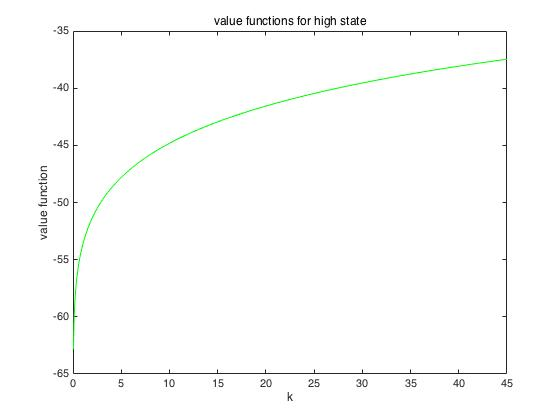
\includegraphics[width=7in,height=4in]{vfnh}
	
	\end{figure}
    \begin{figure}[!h]{\centering}
	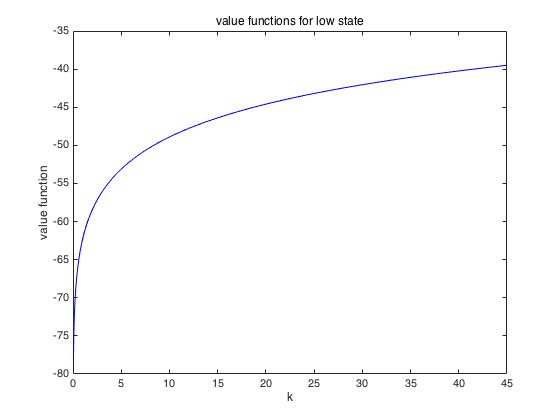
\includegraphics[width=7in,height=4in]{vfnl}
	
    \end{figure}
   \newpage 
   \noindent As we can see from the figure, value functions are increasing and concave. Also, value of value function in high state is bigger, which means value functions are increasing on $\mathcal{A}$ too.
	\\
	\section{Question 3}
	Below is the figure for policy functions, where the green line is for high productivity state and the blue line is for the low productivity state:
	\begin{figure}[!h]{\centering}
		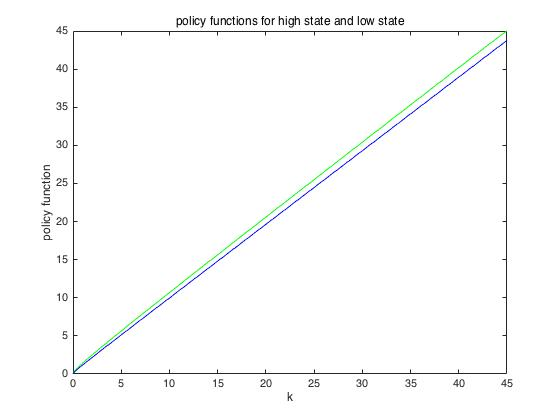
\includegraphics[width=7in,height=2.8in]{pl}
	\end{figure}
    \newline As we can see from the figure above, the policy functions are increasing on both $\mathcal{K}$ and $\mathcal{A}$.
    \section{Question 4}
    I write down the transition matrix and then calculate the invariant distribution using Matlab. Then I get the probabilities for different states in each period, by using Markov chain.\\\\
    After that, I generate a random sequence $r$, and use it to compare with probabolities in each period. If the probability of high state in this period is greater than $r$, then I set $\mathcal{A}$ equals to $\mathcal{A}_h$, otherwise I set $\mathcal{A}$ equals to $\mathcal{A}_l$.\\\\
    Using the above technology shocks to calculate output, and get the standard deviation of output for $\mathcal{A}_h=1.1$ is $0.9126$, which is way too bigger than our desired value 0.018. I try to set different values for $\mathcal{A}_h$, and the minimum for std is 0.076 I can get. Somehing is not right...\\\\
    Please see appendix for Matlab code.
	\section{Question 5}
	I use one equation instead of two to represent the two-state value function. For this quesion, it takes 8 seconds for Matlab to finish, while for question 2 it takes 38 seconds. Get results as below, where green line is for high state and blue line is for low state in both graphs:
	\begin{figure}[!h]\centering
		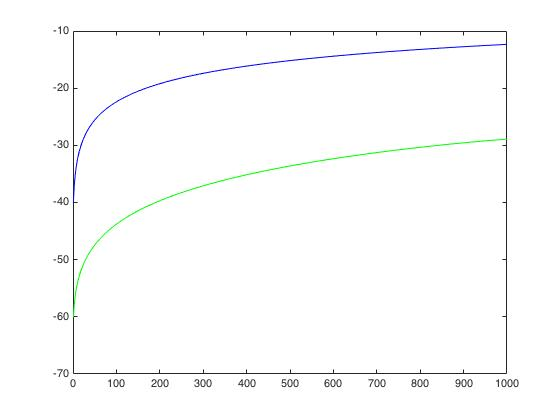
\includegraphics[width=3.2in,height=4in]{vfn_q5}
		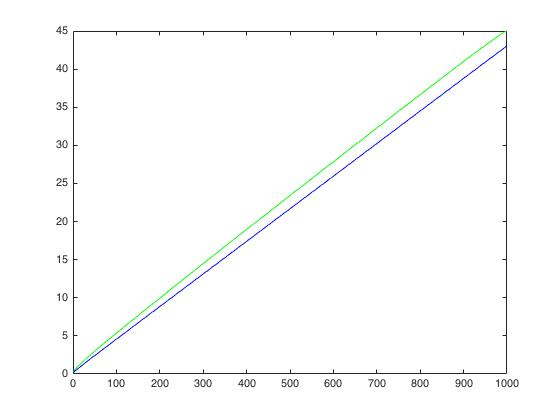
\includegraphics[width=3.2in,height=4in]{pl_q5}
	\end{figure}

	\section{Appendix}
	\subsection{ Steps for VFI}
			\begin{enumerate}
			\item [1.] Deciede on a grid,$\mathscr{K}$, the minimun value I set is 0.2, and the maximun value for k I set is 5. Also there are 20 numbers in k grid $\mathscr{K}$.
			\item [2.] Technology shocks are $A_h$ and $A_l$, together with transition matrix $\prod=\pi_{ij}$.
			\item [3.] For each $k_i\in\mathscr{K}$ and $\ell$ equals l and h, compute the value funcitons.
			\item[4.] Use a loop, which stops when absolute value between $V_{i+1}$ and $V_i$ is less than $\epsilon$.	
		\end{enumerate}
	\subsection{ Matlab code}
	\begin{enumerate}
		\item[1.]Code for Q2 \& Q3\\
  
  
	\begin{verbatim}

	close all
	clear all
	%%%%%%%%parameters%%%%%%%%%%
	delta=0.025;                 %depreciation rate
	alpha=0.35;                  %capital share of production
	beta=0.99;                   %discount rate
	sigma=2;                     %utility function parameter
	pi=[0.977 0.023;0.074 0.926];%transition matrix
	
	%%%%%%%%k grid%%%%%%%%%%%%%%
	ah = 1.1;                    %high productivity 
	al=0.678;                    %low productivity
	knum=1000;                   %set number of k equals 1000
	kmin=0 ;                     %set k min equals 0
	%?*syms kmax
	%?eqn=kmax==ah*kmax^alpha+(1-delta)*kmax
	%?kmax=solve(eqn,kmax)        %calculate the k max[tooooo big
	%kmax = 1.1*(alpha*ah/(1/beta-1+delta))^(alpha/(1-alpha))...
	%+(1-delta)*(alpha*1.1/(1/beta-1+delta))^(1/(1-alpha));
	kmax=45;
	k=linspace(kmin,kmax,knum);  %decide on k grid
	kmat=repmat(k',[1 knum]);    %this is a matrix which will be useful later
	
	%%%%%%%%variables%%%%%%%%%%%
	conh=ah*kmat.^alpha+(1-delta)*kmat-kmat';
	conl=al*kmat.^alpha+(1-delta)*kmat-kmat';
	reth=conh.^(1-sigma)/(1-sigma);
	retl=conl.^(1-sigma)/(1-sigma);
	reth(conh < 0)=-Inf;
	retl(conl < 0)=-Inf;
	
	
	%%%%%%%%Iteration%%%%%%%%%%%
	dis = 1; tol = 1e-06;        % tolerance for stopping 
	v_guess = zeros(2, knum);   %?????
	while dis > tol
	
	vh_mat = reth + beta *(pi(1,1)* repmat(v_guess(1,:), [knum 1])...
	+pi(1,2)*repmat(v_guess(2,:), [knum 1]));
	vl_mat = retl + beta *pi(2,2)* repmat(v_guess(2,:), [knum 1])+...
	beta *pi(2,1)* repmat(v_guess(1,:), [knum 1]);
	
	[vfnh, ph_indxh] = max(vh_mat, [], 2);
	vfnh = vfnh';
	[vfnl, pl_indxl] = max(vl_mat, [], 2);
	vfnl = vfnl';
	
	
	dis =[max(abs(vfnl-v_guess(2,:)));max(abs(vfnh - v_guess(1,:)))]    %?????
	v_guess =[vfnh;vfnl];
	%?????
	
	end
	
	gh = k(ph_indxh);
	gl = k(pl_indxl);
	
	figure
	plot(k,vfnh,'g');
	xlabel('k');
	ylabel('value function');
	title('value functions for high state');
	
	figure
	plot (k,vfnl,'b');
	xlabel('k');
	ylabel('value function');
	title('value functions for low state');
	
	
	figure 
	plot (k, gh,'g');
	xlabel('k');
	ylabel('policy function');
	title('policy functions for high state and low state') ;
	hold on;
	plot(k , gl,'b');
	hold off;
	\end{verbatim}
	
	\item[2.] Code for Q4
	\begin{verbatim}
	close all;
	clear all;
	
	%%%%%%%%parameters%%%%%%%%%%
	delta=0.025;                 %depreciation rate
	alpha=0.35;                  %capital share of production
	beta=0.99;                   %discount rate
	sigma=2;                     %utility function parameter
	pi=[0.977 0.023;0.074 0.926];%transition matrix
	pi_s=pi^1000;                %invariant distribution
	ah=1e-10+1;                  %set a value for high ptoductivity shock
	al=(1-ah*pi_s(1))/pi_s(3);   %calculate low prod shock
	
	%%%%%%%%simulation%%%%%%%%%%
	nStates = 1000;
	initialProbabilityState=[1 0];
	states = zeros(nStates,2);
	states(1,:) = initialProbabilityState;
	for ns = 2:nStates
	states(ns,:) =states(ns-1,:)*pi ;
	end                          %using markov chain to generate a prob seq
	
	for ns=1:nStates
	r=rand();
	if states(ns,1)>r;
	a(ns)=ah;
	else a(ns)=al;
	end
	end                         %get a sequence of a, length of 1000
	
	
	%%%%%%%set k grid%%%%%%%%%%
	knum=1000;                   %set number of k equals 1000
	kmin=0 ;                    
	kmax=45;
	k=linspace(kmin,kmax,knum);  %decide on k grid
	kmat=repmat(k',[1 knum]); 
	
	%%%%%%%std of output%%%%%%
	for ns=1:1000
	y(ns)=a(ns)*k(ns).^alpha;
	y_std=std(y);
	end
	\end{verbatim}
	\item[3.]Code for Q5
	\begin{verbatim}
	close all
	delta=0.025;              %depreciation rate
	alpha=0.35;               %capital share of income
	beta=0.99;                %discount rate
	sigma=2;                  %utility parameter
	
	
	nbk=1000;                 %number of data points int he grid
	nba=2;                    %number of value for the shocks
	crit=1;                   %convergence criterion
	epsi=1e-1;                %convergence parameter
	
	phh=0.977;               %this is pi hh
	pll=0.926;               %p ll
	PI=[phh 1-phh;1-pll,pll]; %transition matrix
	ah=1.1;
	al=0.678;
	A=[ah al];               %stochastic matrix
	
	
	kmin=0.1;
	kmax=45;
	k=linspace(kmin,kmax,nbk)';% k grid
	c=zeros(nbk,nba);
	util=zeros(nbk,nba);
	v=zeros(nbk,nba);
	Tv=zeros(nbk,nba);
	
	
	%%%%%%%%%%%%%%%%%%set up%%%%%%%%%%%%%%%%%%%%%
	
	while crit>epsi
	for i=1:nbk
	for j=1:nba
	c=A(j)*k(i)^alpha+(1-delta)*k(i)-k;
	neg=find(c<0);
	c(neg)=NaN;
	util(:,j)=(c.^(1-sigma))/(1-sigma);
	util(neg,j)=-1e12;
	end
	[Tv(i,:),pl(i,:)]=max(util+beta*(v*PI));
	end
	crit=max(abs(Tv-v));
	v=Tv;
	i=i+1;
	end
	
	gh=k(pl(:,1));
	gl=k(pl(:,2));
	
	figure
	plot(v(:,1),'g-*');
	hold on ;
	xlabel=('k');
	ylabel=('value function');
	title=('value functions');
	plot(v(:,2),'b-o');
	hold off;
	
	figure
	plot(gh,'g-*');
	xlabel=('k');
	ylabel=('policy function');
	title=('policy functions');
	hold on;
	plot(gl,'b-o');
	hold off;
	
	
	
	\end{verbatim}
	\end{enumerate}


	

	
	
	
	
	
	
	
	
	
	
	
	
	
	
	
\end{document}